% !TEX root = ./paper.tex
% Background and motivation

%TODO
%Gives an overview of \tls / \tcp and how they interact. We also need a comparison
%of QUIC and \tls/\tcp on several points that would serve as a base to explain why
%\tls 1.3's extensibility cannot compete with QUIC.
%Gives an overview of \tls / \tcp and how they interact.

%\begin{figure}[!t]
%  \begin{center}
%    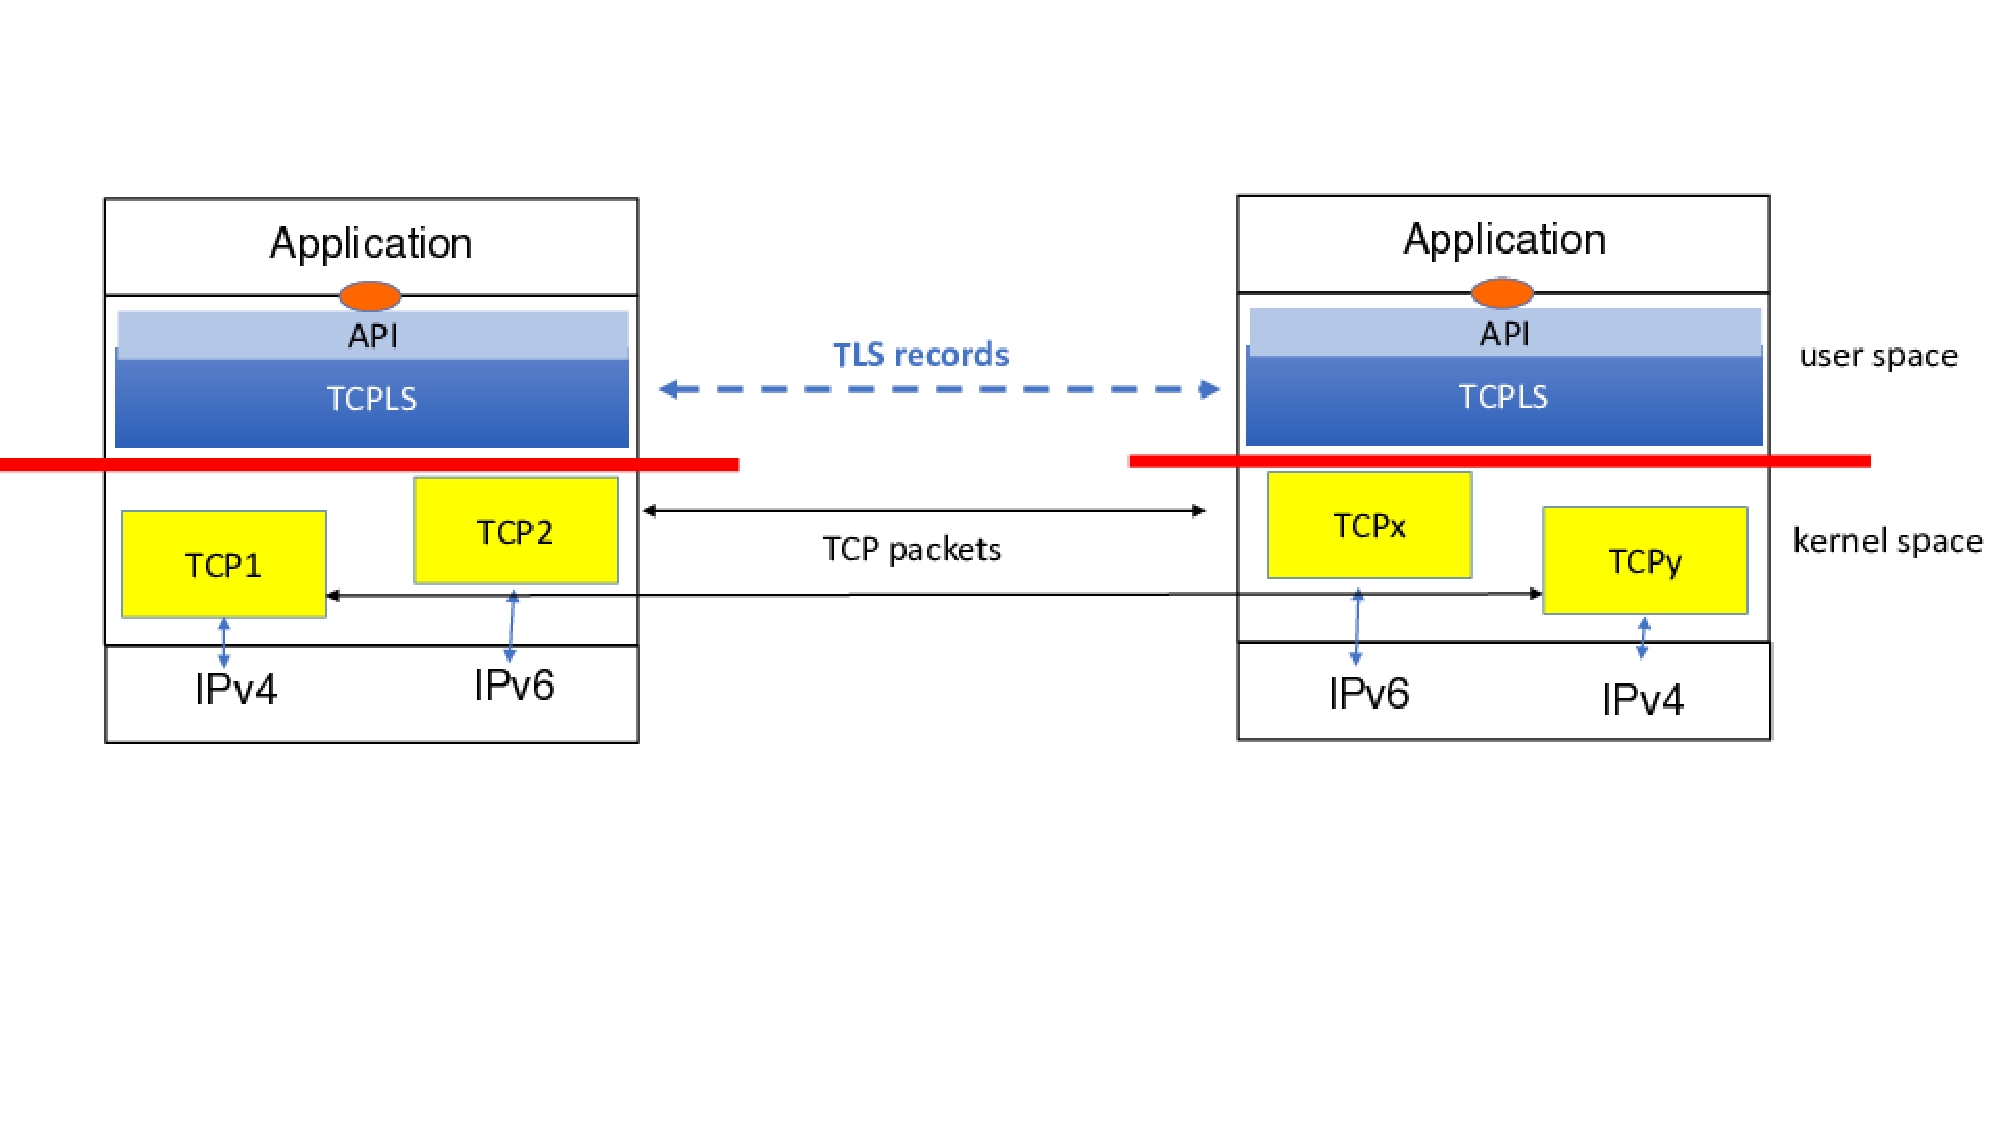
\includegraphics[width=8cm]{figures/tcpls-fig2.pdf}
%  \end{center}
%  \caption{\tcpls in the stack.}
%  \label{fig:arch}
%\end{figure}

The slow pace of innovation in \tcp-based transport services can be explained by 
several factors. First, the amount of bytes for extensions in the \tcp header is
limited to 40 bytes. Second, it is exchanged in cleartext and is known to have heavily
ossified due to middleboxes, strongly restraining changes in the header semantics 
and to \tcp \texttt{Options}. Third, TCP is often implemented in the kernel, 
which adds complexity to implement and deploy these modifications. Following the
recent advances in the transport layer, we go back to {\small{\textit{RQ1}}}
and ask \textit{Can TCP and TLS be combined to address these issues} ?

Yes, by leveraging the
flexible encrypted \tls records, we can supplement the \tls-encrypted application data
with transport-level control data allowing to extend the offered transport services.
Existing \tcp \texttt{Options} can be securely conveyed in new \tls records and 
new transport services can leverage this new secure control channel.

In this section, we explain how we combined \tcp and \tls into \tcpls. We first explain how
a \tcpls connection starts. We introduce
\tcpls records which are the basic unit of communication in \tcpls. We then explain
how they can be leveraged to provide modern transport services such as multiplexing,
connection migration and multipath.


\subsection{\tls Records and Extensions}
%%%%%%%%%%%%%%%%%%%%%%
%Today's applications expect more than a simple bytestream from the transport
%layer. Security is not anymore a requirement for niche application. Applications
%expect secure transport by default. Similarly, applications are not restricted
%anymore on using only one network interface. They need to efficiently deal with
%IPv6 and IPv4 on dual stack hosts and manage the utilization of different
%network interfaces on mobile devices such as smartphones.
%\tcpls provides a
%fast, flexible, and secure transport protocol that is suited for these modern
%applications.

\definecolor{lightgray}{gray}{0.8}
\newcommand{\colorbitbox}[4]{%
	\sbox0{\bitbox[#4]{#2}{#3}}%
	\makebox[0pt][l]{\textcolor{#1}{\rule[-\dp0]{\wd0}{\ht0}}}%
	\bitbox[#4]{#2}{#3}%
}
\begin{figure}
\begin{bytefield}[bitheight=\widthof{abcde}]{24}
	\begin{rightwordgroup}{\tls 1.3 Records}
	\bitbox{8}{\small Opaque Type \\ \scriptsize AppData} & \bitbox{8}{\small TLS Version && \scriptsize \texttt{0x303}} & \bitbox{8}{Length} \\
	%\wordbox[tlr]{2}{Encrypted and \\ authenticated payload} \\
	\colorbitbox{lightgray}{16}{Encrypted payload}{tlb} & \colorbitbox{lightgray}{8}{\small Record type \\ \scriptsize e.g. AppData}{trb}
	\end{rightwordgroup}
\end{bytefield}
\begin{bytefield}[bitheight=\widthof{abcde}]{24}
	\begin{rightwordgroup}{\tcpls Records}
	\bitbox{8}{\small Opaque Type \\ \scriptsize AppData} & \bitbox{8}{\small TLS Version && \scriptsize \texttt{0x303}} & \bitbox{8}{Length} \\
	%\wordbox[tlr]{2}{Encrypted and \\ authenticated payload} \\
	\colorbitbox{lightgray}{16}{\small Encrypted control \\ or app. data}{tlb} & \colorbitbox{lightgray}{8}{\small Record type \\ \scriptsize TCPLS}{trb}
	\end{rightwordgroup}
\end{bytefield}

	\caption{\tcpls extends the encrypted \tls records to convey control and application data.}
	\label{fig:tls-tcpls-records}
\end{figure}

Each protocol has a basic unit for exchanging application and control data.
For instance for \tcp it is \tcp segments which are split in two with only
a small part dedicated to control data.
\tls is more flexible with \tls records of different types and lengths.
In \quic, the basic unit is are \quic packets which can be composed of any number and type
of \quic frames. As illustrated in Figure~\ref{fig:tls-tcpls-records}, in \tcpls we leverage the \tls encrypted records which hide from middleboxes
their true type and content in opaque \texttt{Application Data} records.
In this way, we can extend the messages exchanged with \tls in a secure and
flexible manner.

\todo{Discuss the (performances) advantages of framing our protocol at the record layer?}

\tls also offers a mean for requesting extended functionalities in a \tls session through
request/response messages called \tls \texttt{Extensions}. They are exchanged during
the \tls handshake with some security guarantees. \todo{state them briefly}
\tcpls extends these messages to negotiate the new transport services it offers.

\subsection{Starting a \tcpls connection}

A \tcpls connection starts with a \tcp handshake followed by a \tls handshake.
This process can be safely accelerated through the use of TCP Fast Open~\cite{rfc7413}.
%\tls 1.3~\cite{rfc8446} has been designed with careful consideration for
%potential extensions and to prevent middlebox interference. 
A \tcpls client
indicates its willingness to use \tcpls with the \tcpls \texttt{Hello} extension
in its \tls \textsc{ClientHello} message. Upon reception of this extension, the \tcpls server
replies with a \tls \textsc{ServerHello} message echoing the \tcpls \texttt{Hello} extension in \tls \textsc{EncryptedExtensions}.
%It can opportunistically add
%lightweight \tcpls data and \tcp options as \textsc{EncryptedExtensions}. 
These are encrypted with the handshake key which is not part of the context used to derive the eventual
application key. 
%If the client does not support some extension, it echoes back
%an alert with the value of the option it does not recognize, letting the connection
%continues.
Once the \tls handshake has succeeded, the peers can exchange \tcpls records.

%\todo{Is the following best here? -> Background ?}
%A reasonable approach to design extensibility mechanisms in the Internet
%is to avoid leaking any information that could help an on-path attacker
%recognize specific users or applications. Indeed, censorship~\cite{Morshed2017a,
%	Gosain2017a,Chai2019a} can be easily implemented when protocol messages can be
%distinguished. Researchers advocates that avoiding trivial opportunities to
%implement censorship should become the bare minimum in designing a new protocol.
%\tcpls%'s control protocol 
%considers these problems by restricting the use of
%plaintext extensions data in the \textsc{ClientHello} as much as possible.


%To prevent middlebox interference, the \tls 1.3 Record Protocol ensures that any
%new message appears as an \textsc{AppData} message type. \tls stores the true
%content type (TType) at the end of the encrypted payload. \tcpls uses this
%feature of \tls 1.3 to encode the control messages that are sent over the secure
%channel as new \tls record types.

%\tcpls is more than the simple addition of the security features
%of \tls and the reliability features of \tcp. \tcpls leverages \tls 1.3 to
%negotiate a security context and uses it to send the user data authenticated and
%encrypted as \tls records. These records create a secure
%control channel between the client and server. This channel is used to manage
%the \tcpls session and exchange all control information without any possible
%middlebox interference. \tcpls includes a Connection Manager (CM) that
%controls the underlying \tcp connections. The \tls records of a \tcpls session can
%be transported over different \tcp connections during the session lifetime. This
%brings several interesting failover and multipath capabilities.
%Fig.~\ref{fig:arch} illustrates the interactions between two \tcpls hosts.
%\tcpls can be implemented in userspace within a library like current \tls
%implementations. It interacts with the \tcp stack that in our prototype resides
%in the kernel. The crypto module negotiates and manages the security context
%while the CM manages the utilization of the underlying \tcp connection(s).
%Closely coupling \tcp and \tls in \tcpls brings opportunities for performance improvement (e.g., avoiding records fragmentation with dynamic receive buffer auto-tuning and/or with dynamic control of the record length), and for connection reliability (e.g., failover).



%\begin{figure}[!t]
% \begin{center}
%\begin{tikzpicture}[node distance=0 cm,outer sep = 0pt,inner sep = 2pt,  scale=0.80, transform shape]
%       \tikzset{application/.style={align=center,minimum height=0.3cm,minimum width=10mm}}
%       \tikzset{tcpls/.style={align=center,shape=rectangle,fill=green!70!red!100,minimum height=1.5cm,minimum width=22mm,rounded corners, draw}}
%        \tikzset{conman/.style={align=center,shape=rectangle,fill=blue!70!green!10,minimum height=0.15cm,minimum width=10mm,rounded corners, draw}}
%       \tikzset{api/.style={align=center,shape=rectangle,fill=purple!30,minimum height=0.15cm,minimum width=22mm,rounded corners,draw}}
%       \tikzset{tcp/.style={align=center,shape=rectangle,fill=yellow, minimum height=0.4cm,minimum width=5mm,rounded corners,draw}}
%       \tikzset{label/.style={align=center,minimum height=0.5cm,minimum width=5mm}}
%       \draw(-3,-0.3) rectangle (-0.5,0.4);
%       \draw(-3,-3.8) rectangle (-0.5,0.4);
%       \draw [red, ultra thick] (-3,-2.5) -- (-0.5,-2.5);
%       \draw(-3,-4.5) rectangle (-0.5,-3.8);
%       \draw[fill=red!50] (-1.75,-0.3) ellipse (9pt and 4pt);
%       \node[application, xshift=-18mm](application){Application};
%       \node[tcpls, below= 6.3mm and 0mm of application, xshift=0.3mm](tcpls1){\tcpls};
%       \node[api, name=API, below= 3.0mm and 0mm of application, yshift=0mm, xshift=0.3mm ](api1){API};
%       \node[conman, name=CM, below= 17mm and 0mm of application](cm1){CM};
%       \node[conman, name=CM, below= 7.5mm and 0mm of application](crypto){Crypto};
%       \node[tcp, below= 4.5mm and 0mm of tcpls1, xshift=-6mm](tcpx1){\texttt{TCP}$_1$};
%       \node[tcp, right=5mm and 0mm of tcpx1, yshift=-4mm, xshift=2mm](tcpy1){\texttt{TCP}$_2$};
%       \node[label,  below=8mm and 0mm of tcpx1](ip11){IPV4};
%       \node[label,  below=4mm and 0mm of tcpy1](ip12){IPV6};
%
%
%       \draw(2.3,-0.3) rectangle (4.8,0.4);
%       \draw(2.3,-3.8) rectangle (4.8,0.4);
%       \draw [red, ultra thick] (2.3,-2.5) -- (4.8,-2.5);
%       \draw(2.3,-4.5) rectangle (4.8,-3.8);
%       \draw[fill=red!50] (3.6,-0.3) ellipse (9pt and 4pt);
%       \node[application, right= 0mm and 43mm of application, xshift=-8mm](application2){ Application};
%       \node[tcpls, name=TCPLS, below= 6.3mm and 0mm of application2, xshift=0.3mm](tcpls2){\tcpls};
%       \node[api, name=API, below= 3.0mm and 0mm of application2, , xshift=0.3mm](api2){API};
%       \node[conman, name=CM, below= 17mm and 0mm of application2](cm2){CM};
%       \node[conman, name=CM, below= 7.5mm and 0mm of application2](crypto){Crypto};
%       \node[tcp, below= 4.5mm and 0mm of tcpls2, xshift=6mm](tcpx2){\texttt{TCP}$_x$};
%       \node[tcp, left=5mm and 0mm of tcpx2, yshift=-4mm, xshift=-0.3mm](tcpy2){\texttt{TCP}$_y$};
%       \node[label,  below=8.5mm and 0mm of tcpx2](ip21){IPV4};
%       \node[label,  below=4mm and 0mm of tcpy2](ip22){IPV6};
%
%       \node[label,  below=8mm and 0mm of application2, xshift=15mm,rotate=90 ](user1){user space};
%       \node[label,  below=33mm and 0mm of application2, xshift=15mm, rotate=90 ](user1){kernel space};
%
%       \node[label,  left=of api2, xshift=-5mm, yshift=-5mm, green!70!red!100 ](user1){\tls records};
%       \node[label,  left=of ip22, xshift=-5mm, yshift=10.6mm ](user1){\tcp segments};
%
%       \draw[<->,dotted,green!70!red!100,ultra thick] (tcpls1.east) -- node (line) {} (tcpls2.west);
%       \draw[<->,dotted, ultra thick] (tcpx1.east) -- node (line) {} (tcpx2.west);
%       \draw[<->,dotted, ultra thick] (tcpy1.east) -- node (line) {} (tcpy2.west);
%       \draw[<->, ultra thick] (tcpx1.south) -- node (line) {}(ip11.north);
%       \draw[<->, ultra thick] (tcpy1.south) -- node (line) {}(ip12.north);
%       \draw[<->, ultra thick] (tcpx2.south) -- node (line) {}(ip21.north);
%       \draw[<->, ultra thick] (tcpy2.south) -- node (line) {}(ip22.north);
%       \draw[<->,   thick] (cm1.south) -- node (line) {}(tcpx1.north);
%       \draw[<->,   thick] (cm1.south) -- node (line) {}(tcpy1.north);
%       \draw[<->,   thick] (cm2.south) -- node (line) {}(tcpx2.north);
%       \draw[<->,   thick] (cm2.south) -- node (line) {}(tcpy2.north);
%\end{tikzpicture}
%\end{center}
%\vspace{-0.5cm}
%\caption{\tcpls is implemented as a user space library. The application controls the streams and the underlying \tcp connections through the API. The crypto module manages the security context and the Connection Manager (CM) controls the utilization of one or more \tcp connections using the kernel stack.}
%\label{fig:arch}
%\end{figure}

%\tcp separates control information and data by placing the control information
%in the packet header and the data in the payload. This separation worked well
%until middleboxes started to interfere with \tcp~\cite{10.1145/1064413.1064418,
%  honda2011still}. On a fraction of Internet paths, including e.g., some
%enterprise and cellular networks, some middleboxes interfere by adding,
%removing, or changing \tcp
%options~\cite{wang2011untold,honda2011still,xu2015investigating} and, in some
%cases, also transparently terminating \tcp connections.
%
%%These middleboxes have
%%slowed down the evolution of \tcp in recent years.
%
%\tcpls also uses the packet
%header to exchange \tcp control information, but it leverages the extensibility
%of \tls 1.3 to place control information including some \tcp options inside the
%\tls handshake messages and new \tls records. Since this information is
%encrypted and authenticated, the communicating hosts can exchange new control
%information without encountering middlebox interference. We refer to this
%exchange of control information as the \textit{secure channel} between the two hosts.
%
%A \tcpls session starts with a secure \tls 1.3 handshake~\cite{rfc8446}. The
%client adds a new \tcpls transport parameter in its \textsc{ClientHello}
%message. A \tcpls server replies with a \textsc{ServerHello} message that
%negotiates the security keys and may include additional \tcpls information as
%\textsc{EncryptedExtensions}. After this secure handshake, the client and the
%server have a shared security context.
%
%As \sctp~\cite{rfc4960} or \quic~\cite{draft-ietf-quic-transport}, \tcpls
%supports one or more streams over a single \tcpls session. An application can
%open, attach, and close streams to an existing \tcpls session. Each stream is an
%independent cryptographic context derived from the \tcpls security context. The
%\tcpls streams can carry application data or control information.
%Streams are attached over the Secure Control Channel. Since each stream is an
%independent cryptographic context, the recipient can immediately start to
%decrypt and extract data from the new stream. No round-trip is wasted to attach
%a new stream.
%
%\tcpls' CM controls the utilization of the underlying \tcp connections. It can open, close, or reestablish failed \tcp connections. Each of the connections that composes a \tcpls session is identified by a \emph{transport identifier}. By default, the data from a stream can be sent over any of the underlying \tcp connections. The applications that require finer control over the utilization of the underlying \tcp connections can use the \tcpls API to map a stream on a specific underlying connection. In this case, all the data of this stream is exchanged over this specific connection. By placing two streams on different connections, an application can prevent Head-Of-Line (HOL) blocking among these streams.
%
%\tcpls also supports failover and multipath. To support these features, data
%from a given stream is sent over different \tcp connections. In
%this case, the \tcp level sequence numbers and acknowledgements are not
%sufficient anymore to enable the receiver to reorder the data and \tcpls
%adds its own sequence numbers and acknowledgements that are exchanged as
%new \tls records over the secure control channel. Thanks to these \tcpls acknowledegments, a \tcpls session can survive to the failure of an underlying \tcp connection by reestablishing a new \tcp connection to continue the data transfer and replaying the lost records.
%
%A \tcp connection ends with the exchange of \fin or \rst packets. However, some
%middleboxes force the termination of \tcp connections by sending \rst
%packets~\cite{rfc3360,weaver2009detecting}. \tcpls can preserve established
%session by automatically restarting the underlying \tcp connection upon
%reception of a spurious reset. \tcpls defines the connection termination at the
%stream level: a \tcp connection is closed once the last stream attached to a
%\tcp connection is securely closed.

%In summary, \tcpls provides a flexible abstraction to the
%upper layer that supports various new features such as streams, connection
%reliability, different secure multipath modes, secure connection closing,
%encrypted \tcp options, and leverages \tcp's performance and \tls's state of
%deployment.
